\documentclass[conference]{IEEEtran}
\IEEEoverridecommandlockouts
\usepackage{amsmath,amssymb,amsfonts}
\usepackage{algorithmic}
\usepackage{graphicx}
\usepackage{textcomp}
\usepackage{xcolor}
\usepackage{subcaption}
\usepackage{dirtree}
\usepackage[style=numeric,backend=biber]{biblatex}
\addbibresource{references.bib}
\usepackage{hyperref}
\begin{document}

\title{Deeper Networks for Image Classification}

\author{\IEEEauthorblockN{Alexander Sworski}
\IEEEauthorblockA{\textit{ECS795P – Deep Learning and Computer Vision} \\
\textit{School of Electronic Engineering and Computer Science - Department of Computer Science} \\ {M.Sc. Artificial Intelligence}  \\ 
\textit{Queen Mary University}\\
London, United Kingdom \\
a.sworski@se21.qmul.ac.uk \\
210456914}
}

\maketitle

\begin{abstract}
This paper represents a comparison between different Convolutional Neural Networks. In particular, the models GoogLeNet, VGG-16 and ResNet are compared on different datasets, such as MNIST and Cifar10.
\end{abstract}

\begin{IEEEkeywords}
GoogLeNet, ResNet, VGG-16, MNIST, Image Classification, Deep Learning
\end{IEEEkeywords}

\section{Introduction}
This document is a model and instructions for \LaTeX.
%Please observe the conference page limits. 

\section{Literature Review}

\subsection{Neural Network models}
\subsubsection{GoogLeNet}
GoogLeNet was initially developed as a submission for the ImageNet Large-Scale Visual Recognition Challenge 2014, which it won. The main hallmark of this Model is the improved utilization of the computing resources inside the network. It has 12 times fewer parameters than the winner of 2012 (AlexNet) but performs significantly better. \cite{szegedy_going_2014}
This Model first introduced the idea of an inception module, which can be seen in Figure \ref{fig:x inception module 5x5}.
A second version of the Model was published a year later, which then introduced an improved inception module, which can be seen in Figure \ref{fig:x inception module 3x3}.
This new version reduced computational costs, as bigger convolutions are disproportionately more expensive. Using two 3x3 convolutions instead of 5x5 is computationally less expensive while improving the performance.
Although there are is also a V3 and V4 of GoogLeNet, for this paper, the V2 Inception has been used.
In total the model has 22 layers.
\begin{figure}[!htbp]
     \centering
     \begin{subfigure}[b]{0.25\textwidth}
         \centering
         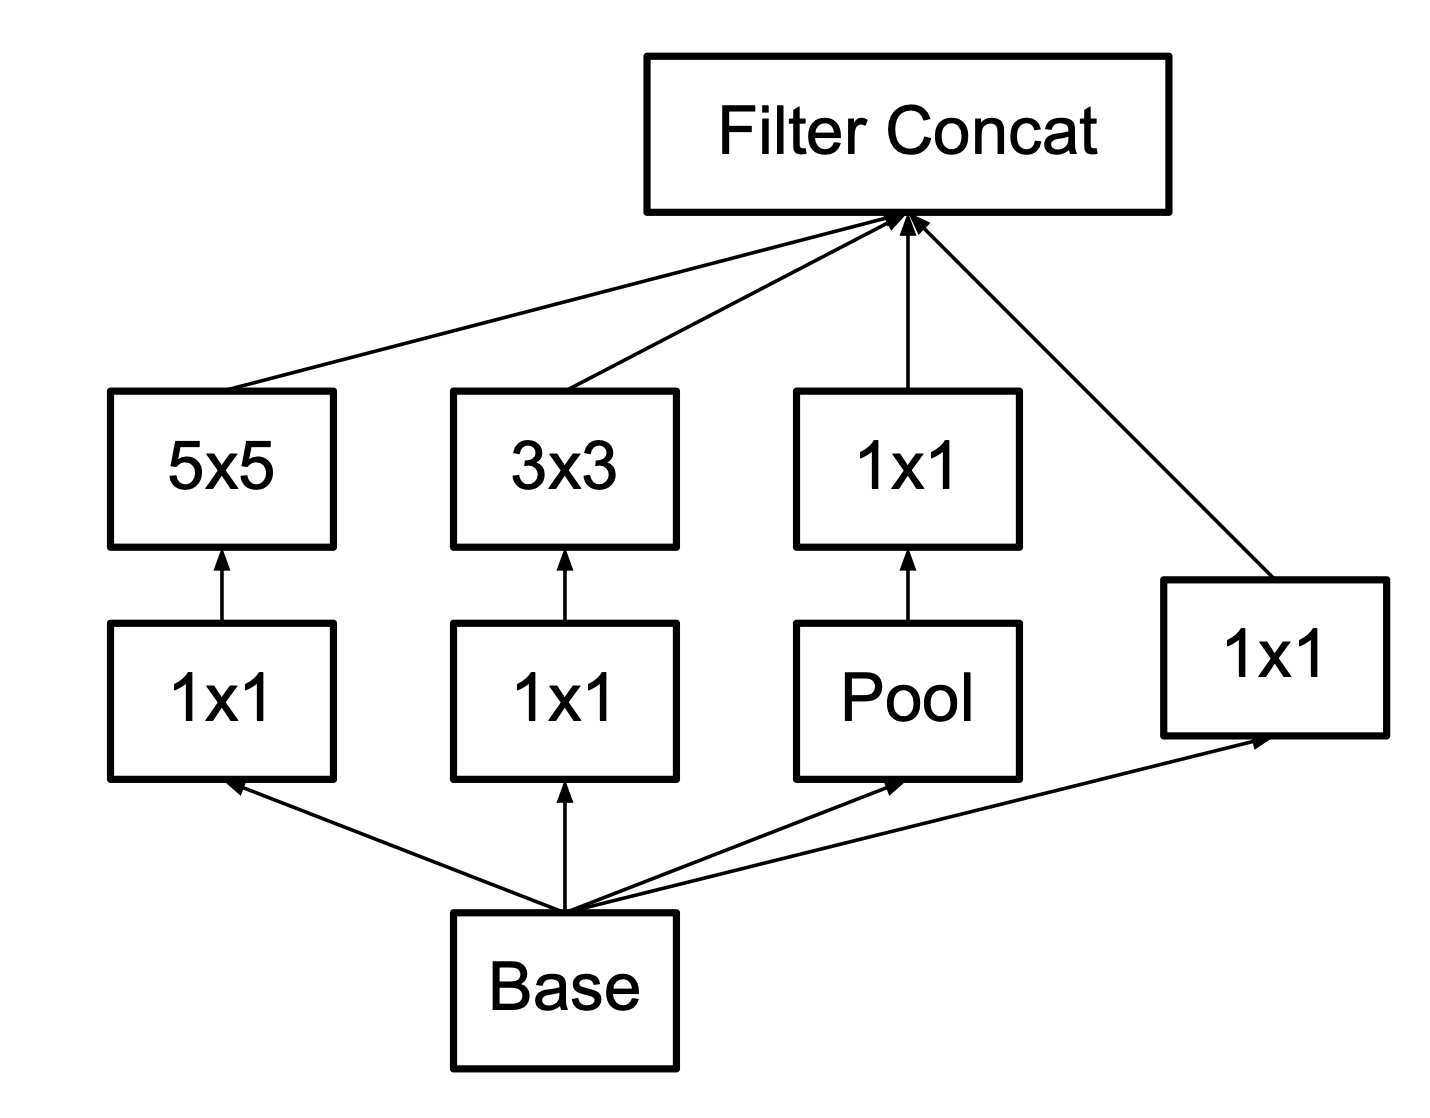
\includegraphics[width=\textwidth]{img/inceptionv1.png}
         \caption{Original Inception module \cite{szegedy_going_2014}}
         \label{fig:x inception module 5x5}
     \end{subfigure}
     \hfill
     \begin{subfigure}[b]{0.22\textwidth}
         \centering
         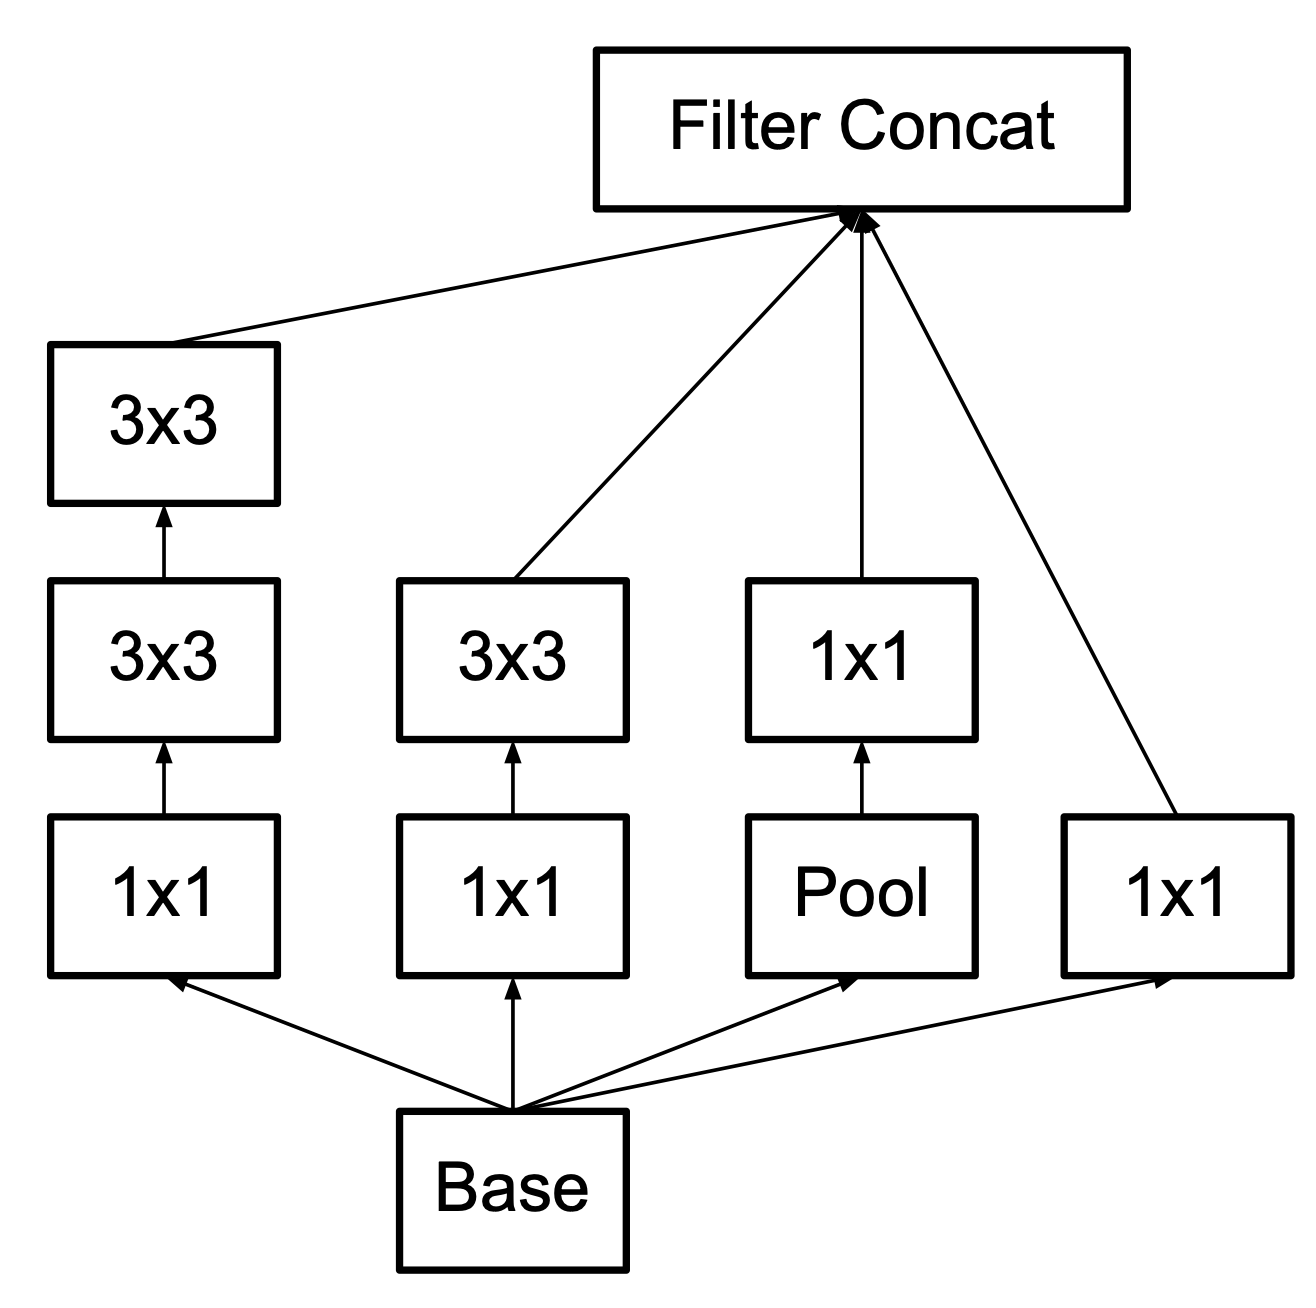
\includegraphics[width=\textwidth]{img/incetionv2.png}
         \caption{V2 Inception module \cite{szegedy_rethinking_2015}}
         \label{fig:x inception module 3x3}
     \end{subfigure}
        \caption{Three simple graphs}
        \label{fig:three graphs}
\end{figure}

\subsubsection{VGG-16}
VGG-16, is the biggest of the models used in this paper (Figure \ref{fig:x mode size}).
It also has been developed as a submission for the ImageNet Challenge, in which it won first and second place for the localization and classification tracks, respectively.
It consists out of 16 layers and uses only 3x3 convolutions. Although it has fewer layers than GoogLeNet, each layer is computationally more complex. Ultimately, this Model resulted in better scores then the GoogLeNet V1 \cite{simonyan_very_2015}.

\begin{figure}[!htbp]
    \centering
    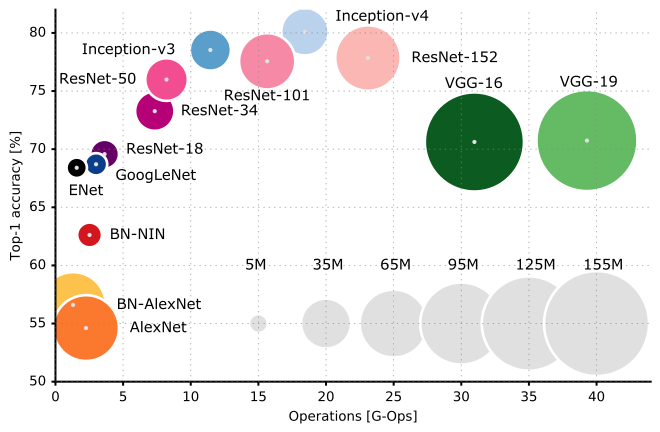
\includegraphics[scale=0.35]{img/model_sizes.png}
    \caption{top-1 one-crop accuracy versus amount of operations required (circle size represents the amount of parameters)}
    \label{fig:x mode size}
\end{figure}

\subsubsection{ResNet}
ResNet, has the highest amount of layers. While there are multiple versions, for this paper a 50 layer version has been chosen.
\begin{figure}[!htbp]
    \centering
    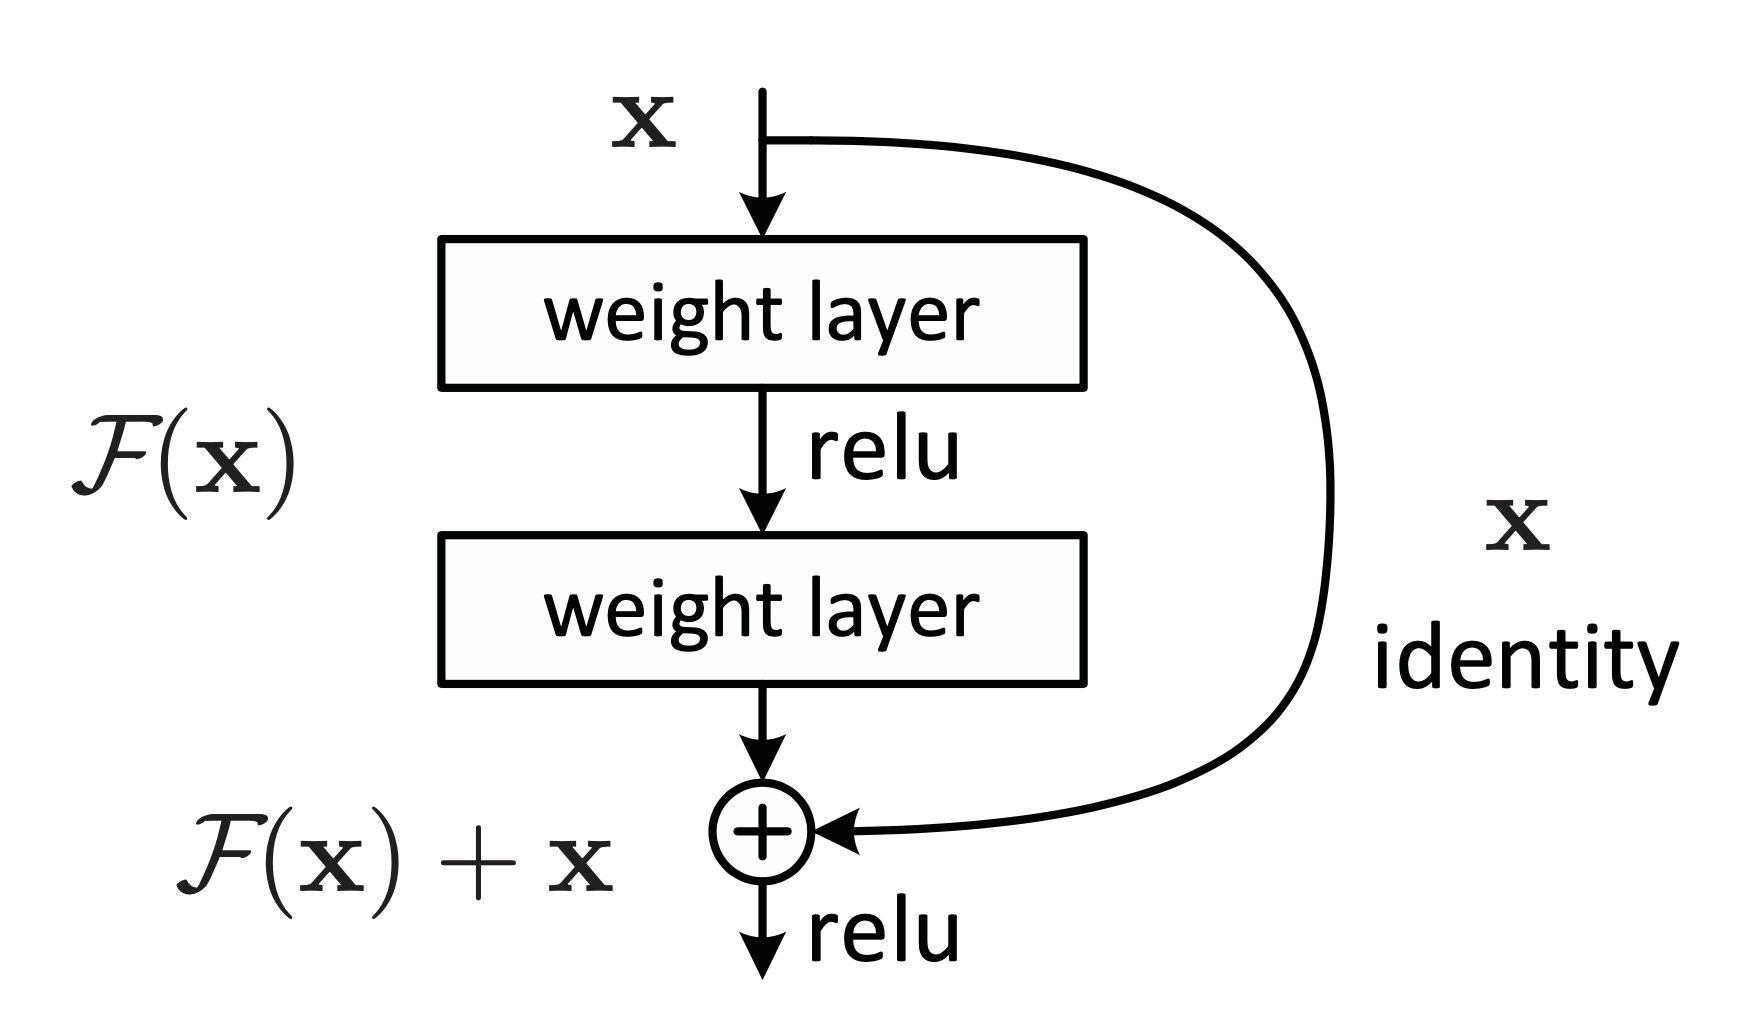
\includegraphics[scale=0.2]{img/residual block.png}
    \caption{Residual learning: a building block \cite{he_deep_2015}}
    \label{fig:x resblock}
\end{figure}
In Figure \ref{fig:x mode size}, it can be observed that the model size is in between GoogLeNet and VGG-16, yet the best result can be expected according to this comparison.
ResNet has been built with the goal of easing the training of deep networks. The network design is based on chaining multiple residual learning blocks on a row. One residual learning block can be seen in Figure \ref{fig:x resblock}. \cite{he_deep_2015}


\subsection{Image datasets}
\subsubsection{MNIST}
The MNIST database contains 70,000 28x28 black and white images. 60,000 images are for training and 10,000 images for testing. The images' portrait handwritten numbers from 0 to 9. \cite{yann_lecun_mnist_nodate} Examples of the classes can be seen in Figure \ref{fig:x MNIST image samples}.
\begin{figure}[!htbp]
    \centering
    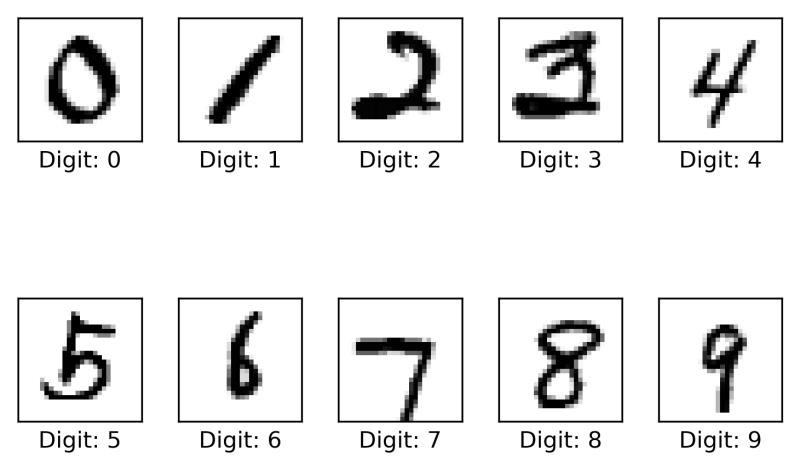
\includegraphics[scale=0.35]{img/mnist_sample.jpeg}
    \caption{Cifar10 image samples \cite{noauthor_convolutional_nodate}}
    \label{fig:x MNIST image samples}
\end{figure}
\subsubsection{Cifar10}
The CIFAR-10 dataset consists of 60000 32x32 colour images in 10 classes, with 6000 images per class. There are 50000 training images and 10000 test images. The classes are mutually exclusive.\cite{noauthor_cifar-10_nodate} Examples of the classes can be seen in Figure \ref{fig:x Cifar10 image samples}.
\begin{figure}[!htbp]
    \centering
    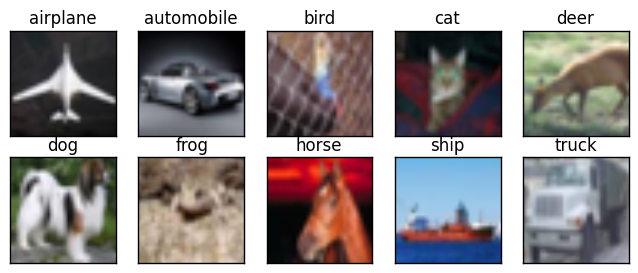
\includegraphics[scale=0.45]{img/cifar_10_sample.png}
    \caption{Cifar10 image samples \cite{noauthor_fig_nodate}}
    \label{fig:x Cifar10 image samples}
\end{figure}

\section{Methodology}
In the first subsection \ref{IM} the implementation of the models using the framework Keras will be explained.
In the subsection \ref{ID} it will be explained how the datasets have been made compatible with the models.
\subsection{Model implementation}\label{IM}
\subsubsection{GoogLeNet}
GoogLeNet considering only the parameters, is the most lightweight Model of the three. Nevertheless, it has 108 operational layers ordered in 22 layers, which can be logically segmented into five stages, excluding input and output. 
The first two stages of the Model consist of multiple 2D convolutions, followed by a \verb|BatchNormalization| layer and a \verb|MaxPooling2D| layer. Using the \verb|BatchNormalization| layer is a unique attribute of the second version of GoogLeNet.
Stage 3 consists of two V2 inceptions, as seen in Figure \ref{fig:x inception module 3x3}, followed by a \verb|MaxPooling2D| layer.
Stage 4 has five inceptions and two auxiliary modules, followed by a \verb|MaxPooling2D| layer. 
In Stage 5, we have two inception modules followed by a \verb|GobalAveragePooling2D| layer, equivalent to the 7x7 convolution found in other versions of this network.
The Model then finishes with a Dropout of 0.4 and a fully connected layer using \verb|softmax| as its activation function.
\cite{szegedy_rethinking_2015}

\subsubsection{ResNet}
...

\subsubsection{VGG-16}
VGG-16 is the biggest Model of the three, regarding the parameters. 
Judging based on layers, this Model is the smallest, as it only consists out of 16 layers, which are segmented into 5 blocks. 
Each block is structured in the same manner. Two or three 2D Convolution, followed by one 2D MaxPolling layer. 
The 5 blocks are then followed by 3 dense layers, one dropout of 0.5 and a final  fully connected layer using \verb|softmax| as its activation function. 
The full network architecture can be seen in Figure \ref{fig:x VGG architecture}. \cite{simonyan_very_2015}

\begin{figure}[!htbp]
    \centering
    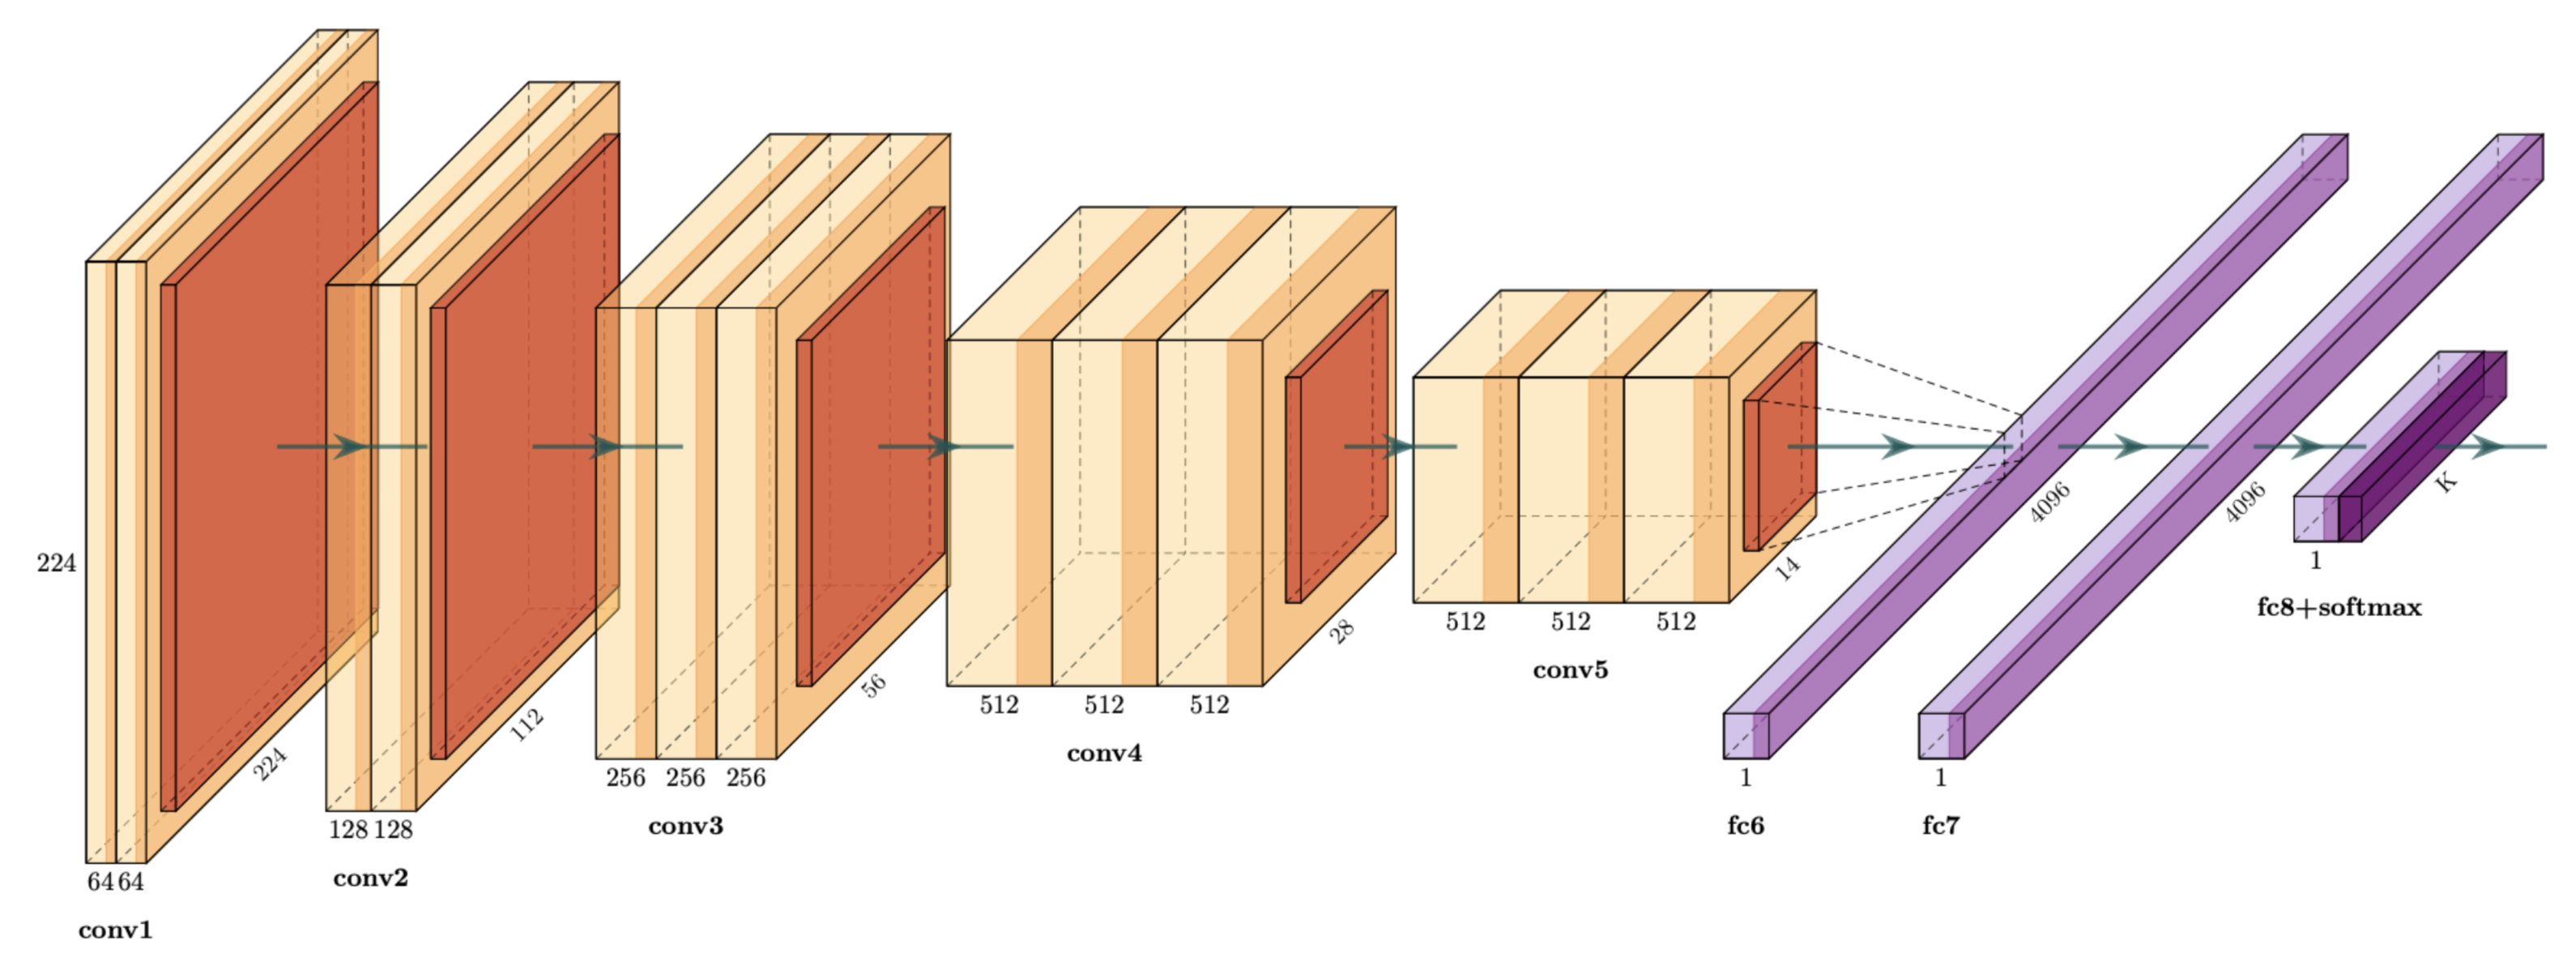
\includegraphics[scale=0.07]{img/VGG.png}
    \caption{VGG-16 architecture \cite{noauthor_forks_nodate}}
    \label{fig:x VGG architecture}
\end{figure}

\subsection{The Datasets}\label{ID}

The dataset used in this paper both have a resolution of 28x28 pixels. On top, the Cifar10 dataset has three colour channels, while the MNIST dataset only has one grey channel.
This represents an issue, as the Neural Networks has initially been designed to work with the Microsoft ImageNet dataset. This dataset has 3 colour channels and a resolution of 224x224 pixels.
The goal was not to change the input of the models, as this would have significant implications for the layers following, resulting in a significant change in the model design.
Therefore, the datasets have been altered as follows to fit the input dimensions of the models.

\subsubsection{MNIST dataset alterations}
The MNIST dataset has the shape (28,28,1), while our models required an input shape of (224,224,3). 
In order to change the dimensionality, the OpenCV library has been used. Using OpenCV, the image has been interpolated to fit the 224x224 image size. 
Afterwards, the image was stacked three times to obtain our three-channel input. Although, there is the OpenCV function \verb|cv2.cvtColor(src, cv2.COLOR_GRAY2RGB)|, 
which can convert from greyscale to RGB. The results are not different from our stacked layers. 
This is due to the unique properties the MNIST dataset has. Using the stacked layers is computational lightweight.

\subsubsection{Cifar10 dataset alterations}
The Cifar10 dataset is already in RGB. Therefore, we do not need to convert it into a different colour space. 
Therefore, this dataset has been interpolated from the shape (28,28,3) to (224,224,3) using the OpenCV library.

\subsection{Project structur}
This project aims to create a GitHub repository that is fully documented and allows for easy replication of the results presented in this paper. 
In Figure \ref{dir: file strucutre}, the file structure of this project can be seen.
All project files, are public on \href{https://github.com/devasworski/Deeper-Networks-for-Image-Classification}{GitHub}.
\begin{figure}[!htbp]
\dirtree{%
 .1 /.
 .2 Checkpoints.
 .3 GoogLeNet.
 .4 CIFAR.
 .5 Adam.
 .5 SGD.
 .4 MNIST.
 .5 Adam.
 .5 SGD.
 .3 ResNet.
 .4 CIFAR.
 .5 Adam.
 .5 SGD.
 .4 MNIST.
 .5 Adam.
 .5 SGD.
 .3 VGG.
 .4 CIFAR.
 .5 Adam.
 .5 SGD.
 .4 MNIST.
 .5 Adam.
 .5 SGD.
 .2 GoogleNet.ipynb.
 .2 VGG.ipynb.
 .2 ResNet.ipynb.
 .2 py.
 .3 ResNet.py.
 .3 googLeNet.py.
 .3 VGG.py.
 .3 helper.py.
 .3 datasets.py.
 .2 Latex.
 .3 Report.tex.
 .3 Report.pdf.
 .3 img.
}
\caption{Project file structure}
\label{dir: file strucutre}
\end{figure}

The project has 3 entry points, which are each a Jupiter Notebook file. Each Notebook is dedicated to one Neural Network.
At the top of the Notebooks, the Hyperparameters of the network can be adjusted as well as runtime environment variables.
The notebooks have two modes, one for a Google Colab execution and one for a local execution.
In case of a Google Colab execution, the notebook will use Google Drive for Checkpoints rather than the Checkpoint folder within the project.
In order to minimize the code within the notebooks and create a clean and easing readable code, code has been outsourced into dedicated python files.
The \verb|helper.py| file, takes care of Hyperparameters as well as evaluating the model. The \verb|dataset.py| handles the dataset download and the alterations described in Section \ref{ID}.
The three other python files define the neural networks, corresponding to their names. Every function within the python files is documented, and the notebooks are divided into descriptive sections.

\section{Results}
Each Model has been trained over 20 epochs twice for each dataset, once using the Adam optimizer and once using the SGD optimizer. 
The overall accuracy and the confusion Matrix have been recorded. In the following chapter, the results will be presented.

\subsection{GoogLeNet}
Using the SGD optimizer, the Model performed very well on the MNIST dataset but was suboptimal on the CIFAR-10 dataset. 
If we look at the confusion matrix of the Model using the SGD optimizer on the CIFAR-10 dataset, we can see that the low accuracy comes from a localized inadequate recognition of the labels bird, cat & deer, which even as a human are very difficult to distinguish from each other.

We can see a significant reduction in accuracy and a double in training speed with the Adam optimizer.
In Figure \ref{fig:GoogLeNet Confusion Matrixis} we can clearly see, that using the Adam optimizer in both cases led to no training at all.

\begin{figure}[!htbp]
    \centering
    \begin{subfigure}[b]{0.22\textwidth}
        \centering
        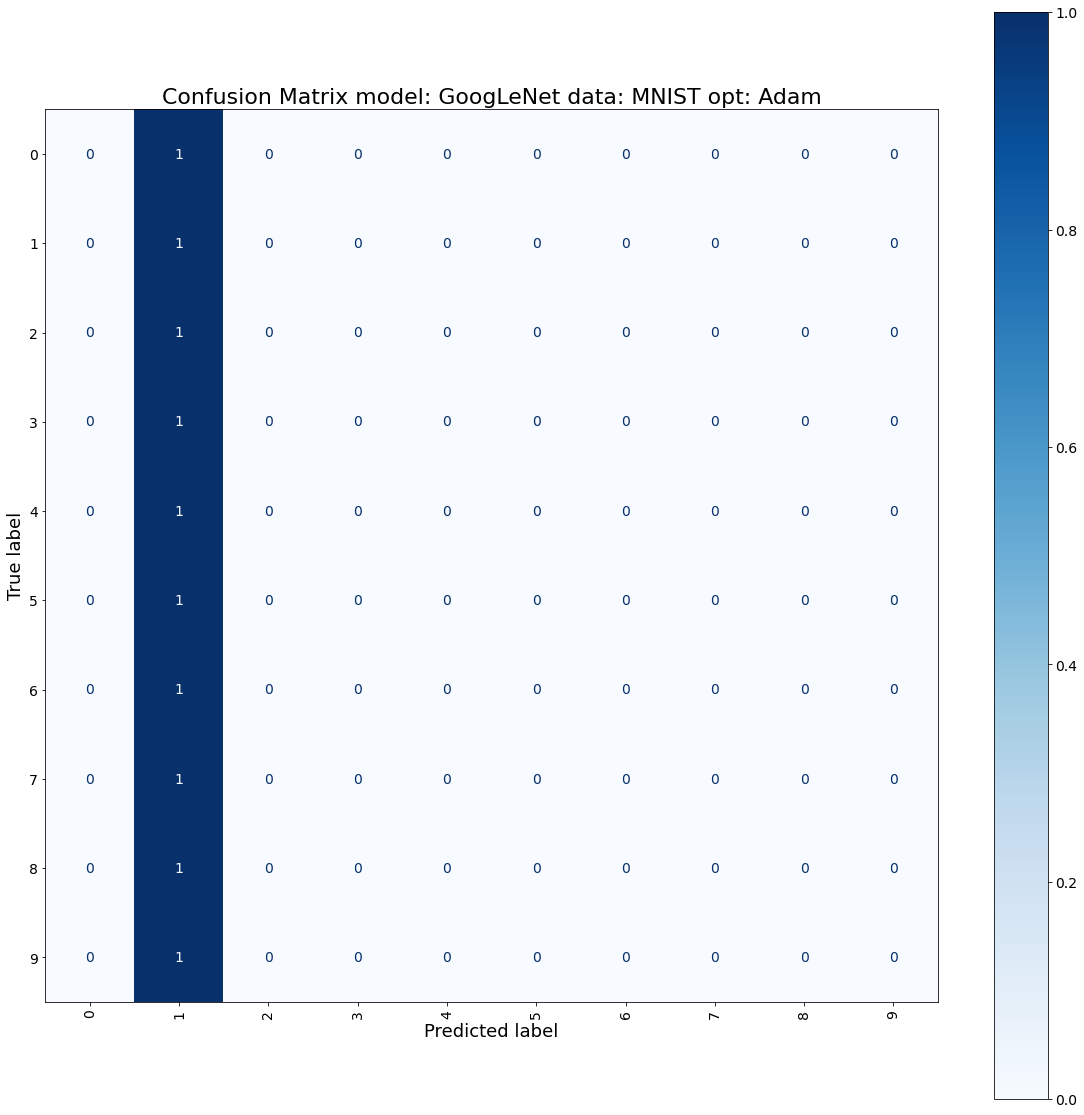
\includegraphics[width=\textwidth]{img/matrx_GoogLeNet_MNIST_Adam.png}
        \caption{Confusion Matrix GoogLeNet MNIST Adam}
        \label{fig:x imatrix_GoogLeNet_MNIST_Adam}
    \end{subfigure}
    \hfill
    \begin{subfigure}[b]{0.22\textwidth}
        \centering
        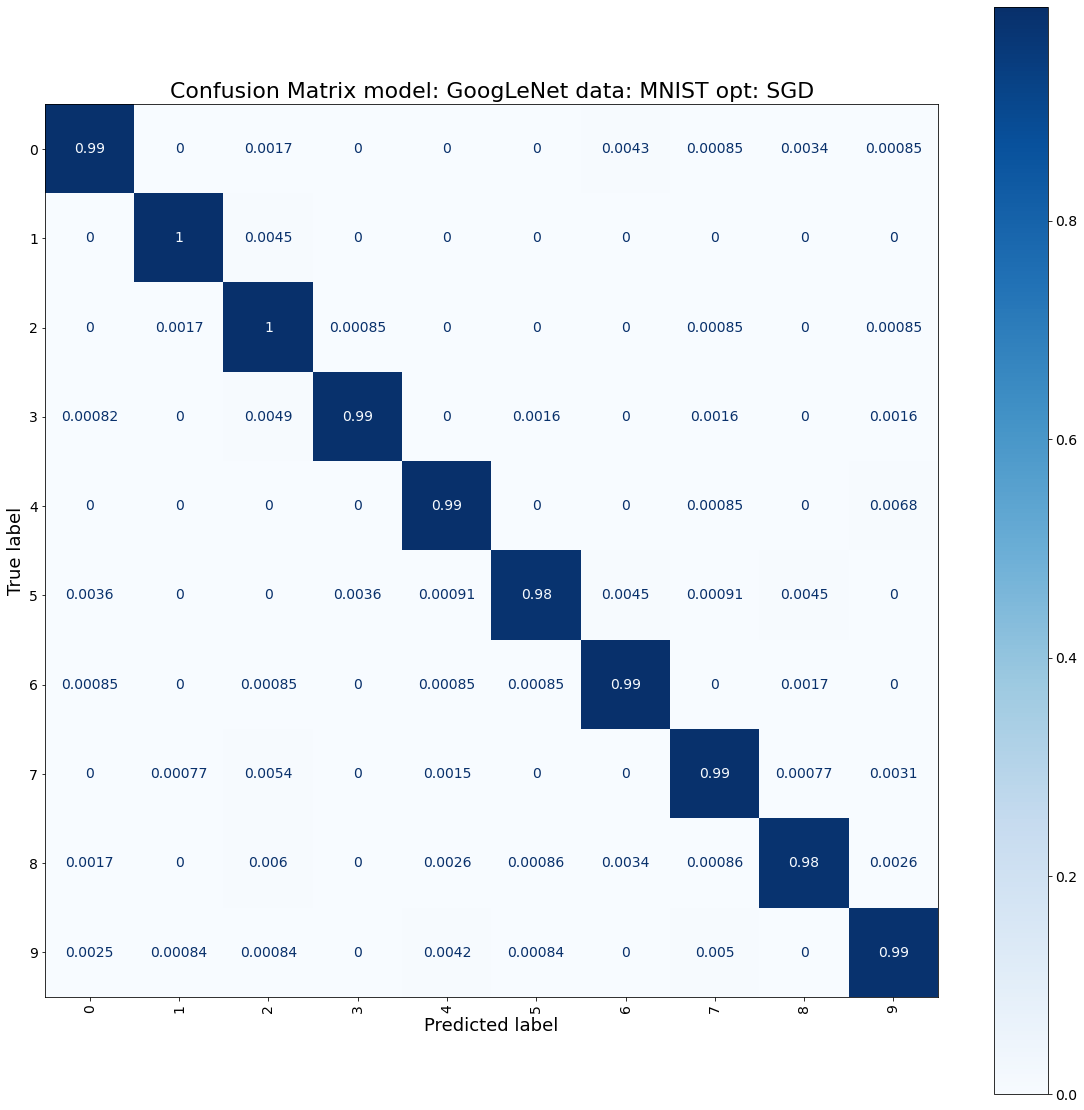
\includegraphics[width=\textwidth]{img/matrix_GoogLeNet_MNIST_SGD.png}
        \caption{Confusion Matrix GoogLeNet MNIST SGD}
        \label{fig:x matrix_GoogLeNet_MNIST_SGD}
    \end{subfigure}
    \begin{subfigure}[b]{0.22\textwidth}
        \centering
        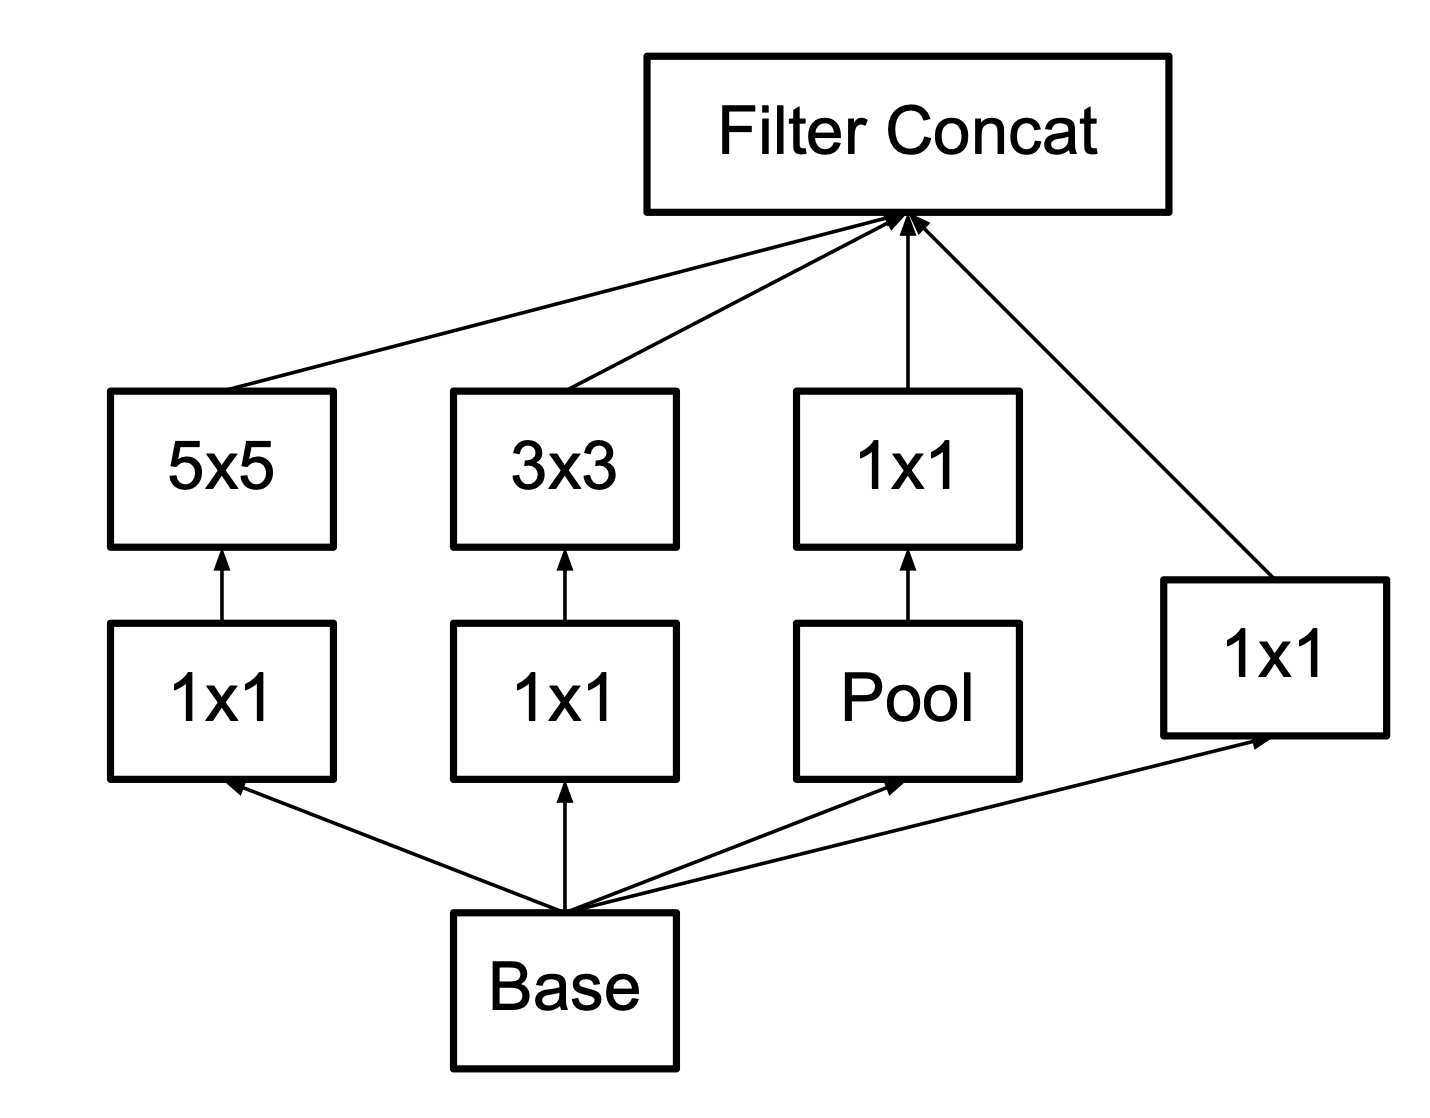
\includegraphics[width=\textwidth]{img/inceptionv1.png}
        \caption{Confusion Matrix GoogLeNet Cifar10 Adam}
        \label{fig:x matrix_GoogLeNet_CIFAR_Adam}
    \end{subfigure}
    \hfill
    \begin{subfigure}[b]{0.22\textwidth}
        \centering
        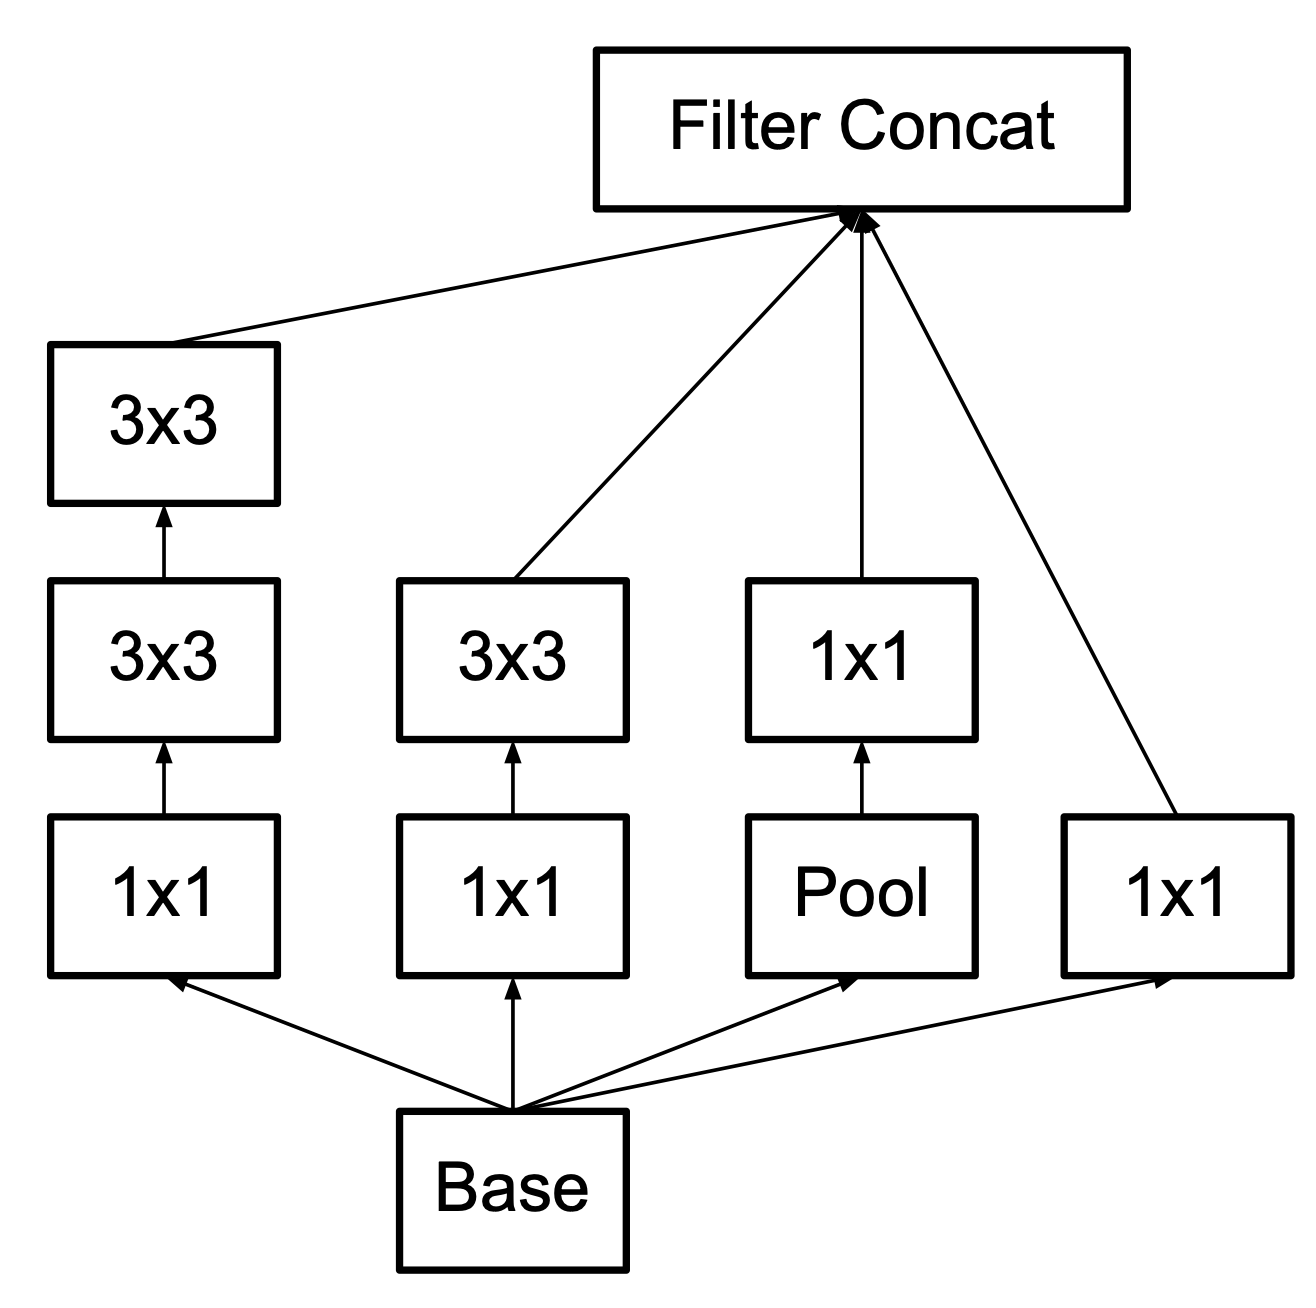
\includegraphics[width=\textwidth]{img/incetionv2.png}
        \caption{Confusion Matrix GoogLeNet Cifar10 SGD}
        \label{fig:x matrix_GoogLeNet_CIFAR_SGD}
    \end{subfigure}
    \caption{Three simple graphs}
    \label{fig:GoogLeNet Confusion Matrixis}
\end{figure}

\begin{table}[htbp]
    \caption{GoogLeNet model accuracy}
    \begin{center}
    \begin{tabular}{|c|c|c|}
    \cline{1-3} 
    \textit{Model accuracy} & \textbf{\textit{Adam}}& \textbf{\textit{SGD}} \\
    \hline
    \textbf{\textit{MNIST}} & 11.02\% & 98.96\% \\
    \hline
    \textbf{\textit{CIFAR-10}} & 10.17\% & 66.34\% \\
    \cline{1-3} 
    \end{tabular}
    \label{tab: GoogLeNet model accuracy}
    \end{center}
\end{table}

\begin{table}[htbp]
    \caption{GoogLeNet training time}
    \begin{center}
    \begin{tabular}{|c|c|c|}
    \cline{1-3} 
    \textit{time/step} & \textbf{\textit{Adam}}& \textbf{\textit{SGD}} \\
    \hline
    \textbf{\textit{MNIST}} & 133s 354ms & 258s 688ms \\
    \hline
    \textbf{\textit{CIFAR-10}} & 110s 351ms & 109s 349ms \\
    \cline{1-3} 
    \end{tabular}
    \label{tab: GoogLeNet training time}
    \end{center}
\end{table}

\subsection{VGG-16}

\begin{table}[htbp]
    \caption{VGG-16 model accuracy}
    \begin{center}
    \begin{tabular}{|c|c|c|}
    \cline{1-3} 
    \textit{Model accuracy} & \textbf{\textit{Adam}}& \textbf{\textit{SGD}} \\
    \hline
    \textbf{\textit{MNIST}} & \% & \% \\
    \hline
    \textbf{\textit{CIFAR-10}} & \% & \% \\
    \cline{1-3} 
    \end{tabular}
    \label{tab: VGG-16 model accuracy}
    \end{center}
\end{table}

\begin{table}[htbp]
    \caption{VGG-16 training time}
    \begin{center}
    \begin{tabular}{|c|c|c|}
    \cline{1-3} 
    \textit{time/step} & \textbf{\textit{Adam}}& \textbf{\textit{SGD}} \\
    \hline
    \textbf{\textit{MNIST}} &  &  \\
    \hline
    \textbf{\textit{CIFAR-10}} &  &  \\
    \cline{1-3} 
    \end{tabular}
    \label{tab: VGG-16 training time}
    \end{center}
\end{table}

\subsection{ResNet-50}

\begin{table}[htbp]
    \caption{ResNet-50 model accuracy}
    \begin{center}
    \begin{tabular}{|c|c|c|}
    \cline{1-3} 
    \textit{Model accuracy} & \textbf{\textit{Adam}}& \textbf{\textit{SGD}} \\
    \hline
    \textbf{\textit{MNIST}} & \% & \% \\
    \hline
    \textbf{\textit{CIFAR-10}} & \% & \% \\
    \cline{1-3} 
    \end{tabular}
    \label{tab: ResNet-50 model accuracy}
    \end{center}
\end{table}

\begin{table}[htbp]
    \caption{ResNet-50 training time}
    \begin{center}
    \begin{tabular}{|c|c|c|}
    \cline{1-3} 
    \textit{time/step} & \textbf{\textit{Adam}}& \textbf{\textit{SGD}} \\
    \hline
    \textbf{\textit{MNIST}} &  &  \\
    \hline
    \textbf{\textit{CIFAR-10}} &  &  \\
    \cline{1-3} 
    \end{tabular}
    \label{tab: ResNet-50 training time}
    \end{center}
\end{table}

\section{Discussion}

\section{Conclusion}

\printbibliography
\end{document}
